\subsection{Internet of Things - network stack}

\begin{itemize}
	\item Write about growing number of devices
	\item how the devices come into play and where they're used.
	\item Describe the devices similarity, that they often are the same. High level of hetrogenous.
\end{itemize}


Write about the growing nubmer if devices. How they're coming into play and where they're used.

\subsubsection{IEEE 802.15.4}
The IEEE 802.15.4 standard intends to offer the fundamental lower network layers for wireless personal area networks (WPAN).  The standard focus is on providing a low cost, low power consumption and low data rates between inexpensive wireless devices. 
The standard only provides the MAC and PHY layers, leaving the upper layers to be chosen by the applicant\cite{6185525} \cite{radio-electronic-802-15-4}. Due to the special PHY layer and to keep the transmission times short and resistant against failures, it does not exchange standard Ethernet frames with maximum transmission unit (MTU) of 1500 octets. The MTU of 802.15.4 is instead set to 127 octets. The communication range is set up to 10 meter and a maximum data transfer rate limited at 250kbit/s. Depending on wireless technology and how constrained the device is, the maximum transmission speed can be set to as low as 20 kbit/s.
[<rewrite this>]
It is important to stress that the 802.15.4 standard does not compete with the regular 802.11 standard, where costs are not as critical and security and speed are more demanded. Today transfer rates up to gigabites is possible with the latest 802.11 standard, these speeds are hardly unneccesary in the IoT domain.[<\/rewrite this>]
\\\\
There are two different types of network nodes that can exist in a 802.15.4 network\cite{radio-electronic-802-15-4}. Full functional device(FFD) and reduced function device(RFD). A FFD node implements all communication funcionallity the 802.15.4 standard offer, it can communicate with any other device in the network. A FFD node may therefore also route data from other nodes. When doing that the node is also called a cooardinator. If all communication in the network is routed through a dedicated FFD node, it is called a PAN coardinatior. A RFD has a reduced level of functionallity and is meant to be extremly simple. Such devices are always an end node in a network and can only communicate through or with a FFD. They can never act as a cooardinator due to their limited capabilities.
\\\\
The two main network topology forms that are used within the 802.15.4 standard, are the star topology and the peer-to-peer topogoly, shown in figure \ref{fig:topology}. In star topology, all devices are required to only communicate to a single central device called the PAN controller. An advantage with this topology is that it makes it easy to manage and support. The drawbacks of using a star topology structure are bigger, for instance will it limit the area that can be covered geographically since all data has to be routed through one device and the distance a node can cover is set to be at a maximum of ten meters.\\
The peer-to-peer topology can have an arbitrary number of connections to each other within the network. Devices can communicate with each other, not only through the PAN controller, with exception for communication between RFDs. There are several advantages by using the peer-to-peer structure, for instance since devices can route traffic via other FFD devices, the network coverage can be easily increased.\\

%picture of the stuff.

\begin{figure}
	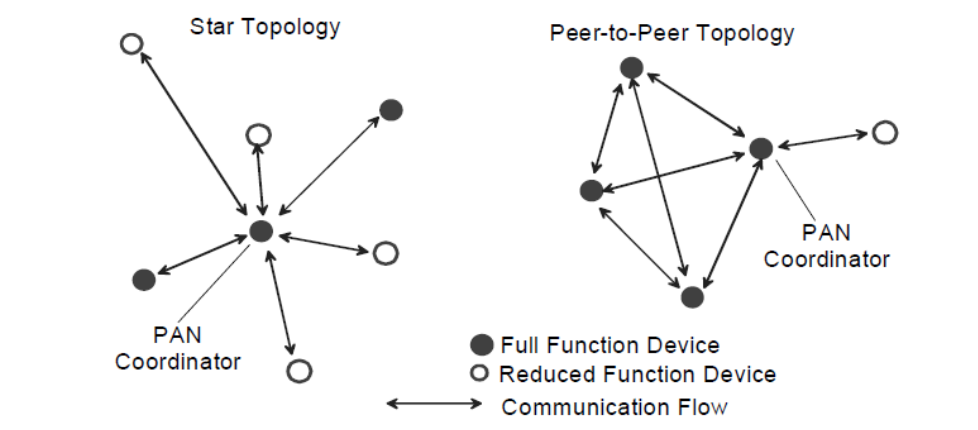
\includegraphics[width=\textwidth]{figures/802-15-4-topologies.png}
	%\caption{Star topology structure on the left, Peer-to-peer on the right. write where it is taken from?}
	\caption{Topology structures in 802.15.4 networks. Star structure on the left, Peer-to-peer on the right.}
	\label{fig:topology}
\end{figure}


% describe the difference and the importance of their functionallites.


exisiting usage of 802.15.4... maybe a subsection of Zigbee too?\\

\subsubsection{IPv4, IPv6}
Since the introduction of Internet Protocol version 4 (IPv4) in 1981\cite{rfc791}, it has been the backbone of the Internet and as the network layer in the OSI model. The protocol defines an address space of 32 bits and the total number of unique addresses that is available with IPv4 is around 4 billion. Today, the IPv4 address space is exhausting at a rapid speed and there is not enough addresses left to handle the increased number of devices that will be connected to the Internet in the future[Make citation!!].
\\\\
In response to the shortage of address space, among other things, the Internet Protocol version 6 (IPv6) was formulised and defined as a successor to IPv4 in 1998\cite{rfc2460}. The IPv6 protocol defines the length of an address of 128 bits, which lead to a total address space of ${2^{128}}$ equal to ${3.4*10^{38}}$ unique addresses. With an address space of this size, it will be sufficient for all IoT and Internet devices to have an own IP address. IPv6 requires that every link to the Internet has an MTU of 1280 octets or greater. In case this need can not be met,  fragmentation and reassembly must be provided at layer below IPv6\cite{rfc2460}.


% Maybee add some more about IPv6?

\subsubsection{6LowPAN}

At first glance, it may seem straightforward to send IPv6 data packets on a 802.15.4 network. However, there are incompabilities between the two formats making it hard for them to cooperate. For instance, the largest frame size of 802.15.4 (127 octets) is considerably less than the required MTU of IPv6 (1280 octets) \cite{rfc4944}. Futhermore, the IPv6 header is 40 octets long which is almost a third of the total 802.15.4 MTU (at least 25 octets). This leaves only 62 octets for upper-layer protocols as UDP or ICMP. That makes it impossible in the first case and infeasable in the second, to build IPv6 direclty on top of the 802.15.4 MAC layer as in a regular IP protocol on the Ethernet MAC layer in the IP stack, shown in figure \ref{fig:ip-6lowpan-stack}.\\\\
To address these issues, among several, ``IPv6 over Low-Power Wireless Personal Area Networks'' (6LoWPAN) was established in 2007 as an adoption layer between the IEEE 802.15.4 MAC-layer and IPv6. 6LowPAN makes it possible to transfer IPv6 packets over a 802.15.4 network through fragmentation and reassembly, and IPv6- and UDP header compressions to shrink the packet size. Through header compression strategies, it is possible to shrink down the IPv6- and UDP header, toward as little as 4 octets in total (instead of 48 octets) \cite{rfc4944}. Other features of 6LowPAN is the neighbor discovery and mesh routing support. Even though there is no limitation to only use UDP, for simplicity and performance reasons it is more favorable to use UDP over TCP as the transport protocol with 6LowPAN.


\begin{figure}
	%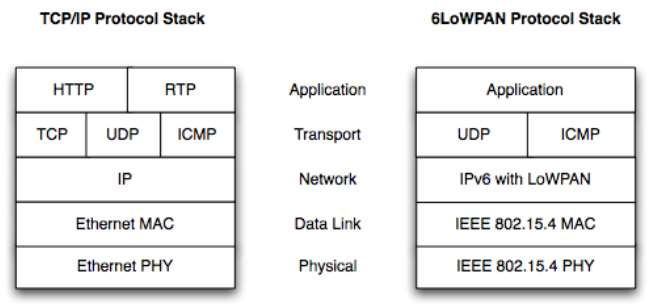
\includegraphics[width=\textwidth]{figures/ip-6lowpan-stack.jpg}
	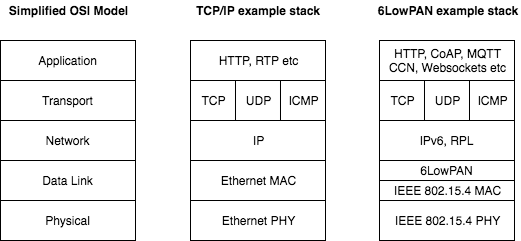
\includegraphics[width=\textwidth]{figures/6lowpan-own.png}
	%\caption{Star topology structure on the left, Peer-to-peer on the right. write where it is taken from?}
	%\caption{Simplified OSI model, an example TCP/IP stack and an illustration of the 6LowPAN protocol stacks, copied from \cite{rfc4944}}
	\caption{The simplified OSI model, an example TCP/IP stack and an illustration of an example 6LowPAN protocol stacks.}
	\label{fig:ip-6lowpan-stack}
\end{figure}

\subsubsection{MQTT, MQTT-SN}
Message Queuing Telemetry Transport(MQTT) is a open lightweight publish-subscribe messageing protocol, designed for constrained devices with low-bandwidth and/or unreliable networks targeting Machine-to-Machine (M2M) communication\cite{mqtt}. The protocol reside in the application layer in the OSI model, assuming that the underlaying network structure provides a point-to-point, session-oriented data transport provided by example TCP/IP \cite{hunkeler2008mqtt}. This assumption makes the protocol unsuitable for devices that can not hold their own TCP/IP stack, which lead to MQTT-SN described further down. The publish-subscribe message pattern require a message broker, which is responsible for distributing messages to the interested clients.
\\\\
The publish-subscribe pattern can be described by a server, or sensor, acting as a publisher/producer of information and a client as the consumer/subscriber of information. A client subscribes on a specific topic, set of data, that resides on the server/sensor. When the server has produced data for the specific topic, it will send that information towards the client. 
The information is going through a broker that handles all the information regarding which devices subscribe to which publisher. The broker is usually located in a traditional network due to its higher performance regarding bandwith and processing capabilities.\\\\
MQTT-SN, where the extension stands for sensor network, is a MQTT version that is adapted for wireless communication. It is optimized to be implemented on low-cost, battery-operated devices with limited or constrained storage and processing capabilities\cite{MQTT-SN}, perticular targeting IoT and sensor devices.\\
Where MQTT uses string characters as topic names, MQTT-SN uses numeric IDs which reduce the size of the packets in favor of readability. Furthermore, MQTT-SN, in contrast to MQTT, does not depend on a connection-oriented transport service (TCP/IP), it is able to work with other transport protocols such as UDP/IP, ZigBee or others. 

[more about brokers and its role.]

\subsubsection{CoAP}
The Constrained Application Protocol (CoAP) is a specialized web transfer protocol to be used with constrained devices and networks, and between M2M communication\cite{rfc7959}. CoAP resides in the application layer, above transport layer, in the OSI model stack.
It provides a client/server interaction model between application endpoints similar to the HTTP standard. 
CoAP is based on the REST architecture and follows the general design to manipulate data in a request/response manner. The methods GET, POST, PUT and DELETE are similar to HTTP, but not identical.
\\\\
While HTTP uses TCP as transportation protocol, CoAP data is sent asynchronously over a datagram-oriented protocol such as UDP. Due to the implementation of UDP, features like resend lost datapackets, and acknowledge-messages are missing in the transport layer[ref kid]. This functionallity has in some extent been moved into the CoAP protocol and is called Messages. \\
CoAP defines four different type of messages: confirmable, non-confirmable, acknowledgment, reset. They occupy 2 bit out of 32 bit of the total CoAP header.
A confirmable message provides reliability by retransmitting a message until a recipient sends an Acknowledgment message with the same Message ID back to the requester. If a requested message can not be handled by the recipient, a reset message will replied instead. When a message does not require reliable transmission (no acknowledgment is needed), a non-confirmable message is sent. These non-confirmable messages will still have a message ID in order to detect duplication.

[note, maybe reorder so first coap, then request/response, then Messages? Add about in network caching? Also add source to second paragraph]












